% Unit: Statistics — running header from here onward
\runningheader{Mathematics 6}{Statistics}{Page \thepage\ of \numpages}

\begingradingrange{stats}
% \subsection*{Section II: Statistics}
% \question[5]
% The weights of all the students in grade 9 are arranged from least to greatest. Which statistical measure separates the top half of this set of data from the bottom half?
% \begin{choices}
%   \choice mean
%   \choice mode
%   \CorrectChoice median
%   \choice average
% \end{choices}
% \begin{solution}
%   The median divides an ordered data set into the lower half and upper half.
% \end{solution}

% \question[5]
% Which statement is true about the data set $3$, $4$, $5$, $6$, $7$, $7$, $10$?
% \begin{choices}
%   \choice mean $=$ mode
%   \choice mean $>$ mode
%   \CorrectChoice mean $=$ median
%   \choice mean $<$ median
% \end{choices}
% \begin{solution}
%   Mean $= \dfrac{42}{7}=6$, median $=6$, mode $=7$.
% \end{solution}

% \question[5]
% Sam's grades on eleven chemistry tests were $90$, $85$, $76$, $63$, $94$, $89$, $81$, $76$, $78$, $69$, and $97$. Which statement is true about the measures of central tendency?
% \begin{choices}
%   \CorrectChoice mean $>$ mode
%   \choice mean $<$ median
%   \choice mode $>$ median
%   \choice median $=$ mean
% \end{choices}
% \begin{solution}
%   Mean $= 81\frac{7}{11}$, median $= 81$, mode $= 76$.
% \end{solution}

% \question[5]
% Which statement is true about the data set $4$, $5$, $6$, $6$, $7$, $9$, $12$?
% \begin{choices}
%   \choice mean $=$ mode
%   \CorrectChoice mode $=$ median
%   \choice mean $<$ median
%   \choice mode $>$ mean
% \end{choices}
% \begin{solution}
%   Mean $= 7$, median $= 6$, mode $= 6$.
% \end{solution}


% \newpage


% \question[5]
% From January 3 to January 7, Buffalo recorded the following daily high temperatures: $5^\circ$, $7^\circ$, $6^\circ$, $5^\circ$, and $7^\circ$. Which statement about the temperatures is true?
% \begin{choices}
%   \CorrectChoice mean $=$ median
%   \choice mean $=$ mode
%   \choice median $=$ mode
%   \choice mean $<$ median
% \end{choices}
% \begin{solution}
%   Mean $= 6$, median $= 6$, modes $= 5$ and $7$.
% \end{solution}

% \question[5]
% The ages of five children in a family are $3$, $3$, $5$, $8$, and $18$. Which statement is true for this group of data?
% \begin{choices}
%   \choice mode $>$ mean
%   \CorrectChoice mean $>$ median
%   \choice median $=$ mode
%   \choice median $>$ mean
% \end{choices}
% \begin{solution}
%   Mean $= 7.4$, median $= 5$, mode $= 3$.
% \end{solution}

% \question[5]
% Melissa's test scores are $75$, $83$, and $75$. Which statement is true about this set of data?
% \begin{choices}
%   \choice mean $<$ mode
%   \choice mode $<$ median
%   \CorrectChoice mode $=$ median
%   \choice mean $=$ median
% \end{choices}
% \begin{solution}
%   Mean $\approx 77.7$, median $= 75$, mode $= 75$.
% \end{solution}



% \newpage


% \question[5]
% The accompanying graph shows the high temperatures in Elmira, New York, for a 5-day period in January.
% \begin{center}
%   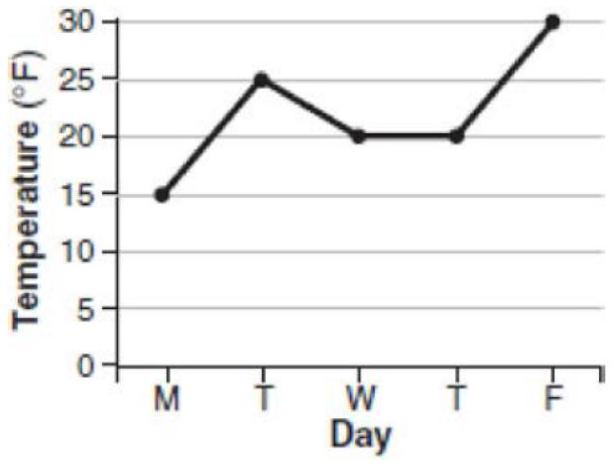
\includegraphics[width=0.5\linewidth]{math-6th/images/2ce67965-b782-401a-ad6e-7a127e5cd380-2_463_613_778_324.jpg}
% \end{center}
% Which statement describes the data?
% \begin{choices}
%   \CorrectChoice median $=$ mode
%   \choice median $=$ mean
%   \choice mean $<$ mode
%   \choice mean $=$ mode
% \end{choices}
% \begin{solution}
%   Answer key: median $=$ mode (read values from the graph to verify).
% \end{solution}

% \question[5]
% Alex earned scores of $60$, $74$, $82$, $87$, $87$, and $94$ on his first six algebra tests. What is the relationship between the measures of central tendency of these scores?
% \begin{choices}
%   \choice median $<$ mode $<$ mean
%   \choice mean $<$ mode $<$ median
%   \choice mode $<$ median $<$ mean
%   \CorrectChoice mean $<$ median $<$ mode
% \end{choices}
% \begin{solution}
%   Mean is $80.\overline{6}$, median is $84.5$, mode is $87$.
% \end{solution}

% \question[5]
% Kelsey scored the following points in her first six basketball games: $22$, $14$, $19$, $22$, $8$, and $17$. What is the relationship between the measures of central tendency of these data?
% \begin{choices}
%   \CorrectChoice mode $>$ median $>$ mean
%   \choice median $>$ mode $>$ mean
%   \choice mean $>$ median $>$ mode
%   \choice mode $>$ mean $>$ median
% \end{choices}
% \begin{solution}
%   Mean is $17$, median is $18$, mode is $22$.
% \end{solution}


% \newpage


% \question[5]
% The test scores for five students were $59$, $60$, $63$, $76$, and $87$. How many points greater than the median is the mean?
% \begin{solutionorbox}[1in]
\end{solutionorbox}
% \begin{solution}
%   Median $= 63$, mean $= \dfrac{59+60+63+76+87}{5} = 69$, so $69-63 = 6$.
% \end{solution}

% \newpage
% \subsection*{Frequency tables, IQR, and open response}
% \question[5]
% On an English examination, two students received scores of $90$, five students received $85$, seven students received $75$, and one student received $55$. The average score on this examination was
% \begin{choices}
%   \choice $75$
%   \choice $76$
%   \choice $77$
%   \CorrectChoice $79$
% \end{choices}
% \begin{solution}
%   $\dfrac{2(90)+5(85)+7(75)+1(55)}{15}=79$.
% \end{solution}

% \question[5]
% What is the mean of the data in the accompanying table?
% \begin{center}
%   \small
%   \begin{tabular}{|c|c|}
%     \hline
%     $x_i$ (scores) & $f_i$ (frequency) \\
%     \hline
%     $25$ & $3$ \\
%     \hline
%     $20$ & $2$ \\
%     \hline
%     $11$ & $5$ \\
%     \hline
%     $10$ & $4$ \\
%     \hline
%   \end{tabular}
% \end{center}
% \begin{choices}
%   \choice $11$
%   \choice $14.5$
%   \CorrectChoice $15$
%   \choice $16$
% \end{choices}
% \begin{solution}
%   $\dfrac{3(25)+2(20)+5(11)+4(10)}{14}=15$.
% \end{solution}

% \question[5]
% The table below gives a set of measures and their respective frequencies. Find the mean of these measures.
% \begin{center}
%   \small
%   \begin{tabular}{|c|c|}
%     \hline
%     Measure $x_i$ & Frequency $f_i$ \\
%     \hline
%     $2$ & $2$ \\
%     \hline
%     $5$ & $3$ \\
%     \hline
%     $7$ & $4$ \\
%     \hline
%     $8$ & $1$ \\
%     \hline
%   \end{tabular}
% \end{center}
% \begin{choices}
%   \choice $5$
%   \choice $5.25$
%   \CorrectChoice $5.5$
%   \choice $6$
% \end{choices}
% \begin{solution}
%   $\dfrac{2(2)+3(5)+4(7)+1(8)}{10}=\dfrac{55}{10}=5.5$.
% \end{solution}


% \newpage



% \question[5]
% What is the mean for the following set of data?
% \begin{center}
%   \small
%   \begin{tabular}{|c|c|}
%     \hline
%     Measure $x_i$ & Frequency $f_i$ \\
%     \hline
%     $70$ & $2$ \\
%     \hline
%     $80$ & $3$ \\
%     \hline
%     $90$ & $5$ \\
%     \hline
%   \end{tabular}
% \end{center}
% \begin{choices}
%   \choice $80$
%   \choice $82$
%   \CorrectChoice $83$
%   \choice $85$
% \end{choices}
% \begin{solution}
%   $\dfrac{2(70)+3(80)+5(90)}{10}=83$.
% \end{solution}

% \question[5]
% What is the median of the set of data shown in the table below?
% \begin{center}
%   \small
%   \begin{tabular}{|c|c|}
%     \hline
%     Measure $x_i$ & Frequency $f_i$ \\
%     \hline
%     $4$ & $15$ \\
%     \hline
%     $5$ & $8$ \\
%     \hline
%     $6$ & $13$ \\
%     \hline
%     $7$ & $10$ \\
%     \hline
%   \end{tabular}
% \end{center}
% \begin{choices}
%   \choice $15$
%   \choice $10.5$
%   \CorrectChoice $5.5$
%   \choice $4$
% \end{choices}
% \begin{solution}
%   There are $46$ values; the median is the average of the $23$rd and $24$th values, which are $5$ and $6$, so median $=5.5$.
% \end{solution}

% \question[5]
% The accompanying table represents the number of cell phone minutes used for one week by $23$ users.
% \begin{center}
%   \small
%   \begin{tabular}{|c|c|}
%     \hline
%     Minutes & Users \\
%     \hline
%     $71$--$80$ & $10$ \\
%     \hline
%     $61$--$70$ & $7$ \\
%     \hline
%     $51$--$60$ & $2$ \\
%     \hline
%     $41$--$50$ & $3$ \\
%     \hline
%     $31$--$40$ & $1$ \\
%     \hline
%   \end{tabular}
% \end{center}
% Which interval contains the median?
% \begin{choices}
%   \choice $41$--$50$
%   \choice $51$--$60$
%   \CorrectChoice $61$--$70$
%   \choice $71$--$80$
% \end{choices}
% \begin{solution}
%   The median is the $12$th user when counts are accumulated from the bottom interval upward; it falls in the $61$--$70$ range.
% \end{solution}


% \newpage



% \question[5]
% What is the median for the following set of data?
% \begin{center}
%   \small
%   \begin{tabular}{|c|c|}
%     \hline
%     $x_i$ & $f_i$ \\
%     \hline
%     $20$ & $2$ \\
%     \hline
%     $21$ & $5$ \\
%     \hline
%     $23$ & $4$ \\
%     \hline
%     $24$ & $4$ \\
%     \hline
%   \end{tabular}
% \end{center}
% \rightfillin{$23$}
% \begin{solution}
%   There are $15$ data values; the $8$th ordered value is $23$.
% \end{solution}

% \question[5]
% What is the mode of the data shown in the following table?
% \begin{center}
%   \small
%   \begin{tabular}{|c|c|}
%     \hline
%     Measure $x_i$ & Frequency $f_i$ \\
%     \hline
%     $5$ & $3$ \\
%     \hline
%     $12$ & $2$ \\
%     \hline
%     $13$ & $5$ \\
%     \hline
%     $18$ & $4$ \\
%     \hline
%   \end{tabular}
% \end{center}
% \begin{choices}
%   \choice $12$
%   \choice $12.5$
%   \CorrectChoice $13$
%   \choice $51.5$
% \end{choices}
% \begin{solution}
%   The value $13$ has the highest frequency ($5$).
% \end{solution}

% \question[5]
% The table below shows five numbers and their frequency of occurrence.
% \begin{center}
%   \small
%   \begin{tabular}{|c|c|}
%     \hline
%     Number & Frequency \\
%     \hline
%     $5$ & $9$ \\
%     \hline
%     $7$ & $5$ \\
%     \hline
%     $8$ & $8$ \\
%     \hline
%     $12$ & $8$ \\
%     \hline
%     $14$ & $8$ \\
%     \hline
%   \end{tabular}
% \end{center}
% The interquartile range for these data is
% \begin{choices}
%   \choice $7$
%   \CorrectChoice $5$
%   \choice $7$ to $12$
%   \choice $6$ to $13$
% \end{choices}
% \begin{solution}
%   With ordered data, $Q_1=7$ and $Q_3=12$, so $\mathrm{IQR}=12-7=5$.
% \end{solution}

% \newpage




% \question[5]
% Which correctly compares the mean and median of the set of data shown in the accompanying table?
% \begin{center}
%   \small
%   \begin{tabular}{|c|c|}
%     \hline
%     $x_i$ & $f_i$ \\
%     \hline
%     $60$ & $2$ \\
%     \hline
%     $75$ & $4$ \\
%     \hline
%     $80$ & $1$ \\
%     \hline
%     $90$ & $3$ \\
%     \hline
%   \end{tabular}
% \end{center}
% \begin{choices}
%   \choice The mean and median are equal.
%   \CorrectChoice The mean exceeds the median by $2$.
%   \choice The median exceeds the mean by $2$.
%   \choice The mean exceeds the median by $2.5$.
% \end{choices}
% \begin{solution}
%   Mean $=77$, median $=75$, so mean exceeds median by $2$.
% \end{solution}


% \question[5]
% Using the data in the accompanying table, which statement is true?
% \begin{center}
%   \small
%   \begin{tabular}{|c|c|}
%     \hline
%     measure $x_i$ & frequency $f_i$ \\
%     \hline
%     $8$ & $1$ \\
%     \hline
%     $10$ & $3$ \\
%     \hline
%     $14$ & $2$ \\
%     \hline
%   \end{tabular}
% \end{center}
% \begin{choices}
%   \choice mean $=$ median
%   \CorrectChoice mean $>$ median
%   \choice mean $<$ mode
%   \choice median $>$ mode
% \end{choices}
% \begin{solution}
%   Mean $=11$, median $=10$, mode $=10$, so mean $>$ median.
% \end{solution}

% \question[5]
% Mrs.\ Porter recorded her students' grades in the frequency table below.
% \begin{center}
%   \small
%   \begin{tabular}{|c|c|}
%     \hline
%     Score & Frequency \\
%     \hline
%     $96$ & $2$ \\
%     \hline
%     $92$ & $5$ \\
%     \hline
%     $88$ & $3$ \\
%     \hline
%     $84$ & $2$ \\
%     \hline
%     $78$ & $4$ \\
%     \hline
%     $60$ & $1$ \\
%     \hline
%   \end{tabular}
% \end{center}
% Which statement is true for the data?
% \begin{choices}
%   \choice mean $>$ median $>$ mode
%   \choice mean $>$ mode $>$ median
%   \CorrectChoice mode $>$ median $>$ mean
%   \choice median $>$ mean $>$ mode
% \end{choices}
% \begin{solution}
%   Mean $\approx 86$, median $=88$, mode $=92$.
% \end{solution}

% \newpage




% \question[10]
% The values of $11$ houses on Washington St.\ are shown in the table below.
% \begin{center}
%   \small
%   \begin{tabular}{|c|c|}
%     \hline
%     Value per house & Number of houses \\
%     \hline
%     $\$100{,}000$ & $1$ \\
%     \hline
%     $\$175{,}000$ & $5$ \\
%     \hline
%     $\$200{,}000$ & $4$ \\
%     \hline
%     $\$700{,}000$ & $1$ \\
%     \hline
%   \end{tabular}
% \end{center}
% Find the mean value of these houses in dollars. Find the median value of these houses in dollars. State which measure of central tendency, the mean or the median, best represents the values of these $11$ houses. Justify your answer.
% \begin{solutionorbox}[1.2in]
\end{solutionorbox}
% \begin{solution}
%   Mean $\approx \$225{,}000$ (exactly $\$2475000/11$). Median $=\$175{,}000$. The median is often better here because one very expensive home pulls the mean up; the median is closer to most house values.
% \end{solution}

% \question[10]
% The prices of seven race cars sold last week are listed in the table below.
% \begin{center}
%   \small
%   \begin{tabular}{|c|c|}
%     \hline
%     Price per race car & Number of race cars \\
%     \hline
%     $\$126{,}000$ & $1$ \\
%     \hline
%     $\$140{,}000$ & $2$ \\
%     \hline
%     $\$180{,}000$ & $1$ \\
%     \hline
%     $\$400{,}000$ & $2$ \\
%     \hline
%     $\$819{,}000$ & $1$ \\
%     \hline
%   \end{tabular}
% \end{center}
% What is the mean value of these race cars, in dollars? What is the median value of these race cars, in dollars? State which of these measures of central tendency best represents the value of the seven race cars. Justify your answer.
% \begin{solutionorbox}[1.2in]
\end{solutionorbox}
% \begin{solution}
%   Mean $=\$315{,}000$. Median $=\$180{,}000$. The median is less affected by the extreme high prices and better reflects a ``typical'' car in this small set.
% \end{solution}

% \newpage
% \subsection*{Range, IQR, and data transformations}

% \question[5]
% What is the range for the following data?
% \[
%   52,\ 32,\ 61,\ 82,\ 63
% \]
% \begin{choices}
%   \CorrectChoice $50$
%   \choice $58$
%   \choice $11$
%   \choice $61$
% \end{choices}
% \begin{solution}
%   Range $= 82 - 32 = 50$.
% \end{solution}

% \question[5]
% Find the range of the following data:
% \[
%   72,\ 89,\ 41,\ 89,\ 73,\ 72,\ 91
% \]
% \begin{choices}
%   \choice $48$
%   \CorrectChoice $50$
%   \choice $52$
%   \choice $58$
% \end{choices}
% \begin{solution}
%   Range $= 91 - 41 = 50$.
% \end{solution}

% \question[5]
% What was the median high temperature in Middletown during the $7$-day period shown in the table below?
% \begin{center}
%   \small
%   \begin{tabular}{|l|c|}
%     \hline
%     \multicolumn{2}{|c|}{Daily high temperature in Middletown} \\
%     \hline
%     Day & Temp.\ (${}^\circ\mathrm{F}$) \\
%     \hline
%     Sunday & $68$ \\
%     \hline
%     Monday & $73$ \\
%     \hline
%     Tuesday & $73$ \\
%     \hline
%     Wednesday & $75$ \\
%     \hline
%     Thursday & $69$ \\
%     \hline
%     Friday & $67$ \\
%     \hline
%     Saturday & $63$ \\
%     \hline
%   \end{tabular}
% \end{center}
% \begin{choices}
%   \CorrectChoice $69$
%   \choice $70$
%   \choice $73$
%   \choice $75$
% \end{choices}
% \begin{solution}
%   Ordered: $63,67,68,69,73,73,75$; median $= 69$.
% \end{solution}


% \newpage



% \question[5]
% The set of numbers $\{4,7,12\}$ has
% \begin{choices}
%   \choice a range of $3$ and a median of $7$
%   \CorrectChoice a range of $8$ and a median of $7$
%   \choice a range of $12$ and a median of $7\frac{2}{3}$
%   \choice a range of $8$ and a median of $7\frac{2}{3}$
% \end{choices}
% \begin{solution}
%   Range $= 12-4 = 8$; median $= 7$.
% \end{solution}


% \question[5]
% Seth bought a used car that had been driven $20{,}000$ miles. After he owned the car for $2$ years, the total mileage of the car was $49{,}400$. Find the average number of miles he drove each month during those $2$ years.
% \begin{solutionorbox}[1.1in]
\end{solutionorbox}
% \begin{solution}
%   $\dfrac{49{,}400 - 20{,}000}{2 \times 12} = \dfrac{29{,}400}{24} = 1{,}225$ miles per month.
% \end{solution}

% \question[10]
% Sara's test scores in mathematics were $64$, $80$, $88$, $78$, $60$, $92$, $84$, $76$, $86$, $78$, $72$, and $90$. Determine the mean, the median, and the mode of Sara's test scores.
% \begin{solutionorbox}[1.8in]
\end{solutionorbox}
% \begin{solution}
%   Mean $= 79$, median $= 79$, mode $= 78$.
% \end{solution}

% \newpage




% \question[10]
% The heights, in inches, of $10$ high school varsity basketball players are $78$, $79$, $79$, $72$, $75$, $71$, $74$, $74$, $83$, and $71$. Find the interquartile range of this data set.
% \begin{solutionorbox}[1.8in]
\end{solutionorbox}
% \begin{solution}
%   Ordered: $71,71,72,74,74,75,78,79,79,83$. With $Q_1 = 72$ and $Q_3 = 79$, $\mathrm{IQR} = 79 - 72 = 7$.
% \end{solution}





% \question[10]
% The following is a list of the individual points scored by all twelve members of the Webster High School basketball team at a recent game:
% \[
%   2,\ 2,\ 3,\ 4,\ 6,\ 7,\ 9,\ 10,\ 10,\ 11,\ 12,\ 14
% \]
% Find the interquartile range for this set of data.
% \begin{solutionorbox}[2in]
\end{solutionorbox}
% \begin{solution}
%   $Q_1 = 3.5$, $Q_3 = 10.5$, so $\mathrm{IQR} = 10.5 - 3.5 = 7$.
% \end{solution}

% \question[5]
% Mr.\ Taylor raised all his students' scores on a recent test by five points. How were the mean and the range of the scores affected?
% \begin{choices}
%   \choice The mean increased by five and the range increased by five.
%   \CorrectChoice The mean increased by five and the range remained the same.
%   \choice The mean remained the same and the range increased by five.
%   \choice The mean remained the same and the range remained the same.
% \end{choices}
% \begin{solution}
%   Adding a constant shifts the mean by that constant but does not change the spread (range).
% \end{solution}


% \newpage



% \question[5]
% If each member of the data set $\{2,2,3,5,8\}$ is multiplied by $2$, which changes will take place in the mean, median, and mode of the data?
% \begin{choices}
%   \CorrectChoice The mean, median, and mode will be multiplied by $2$.
%   \choice The median will remain the same; the mean and mode will be multiplied by $2$.
%   \choice The mode will remain the same; the mean and median will be multiplied by $2$.
%   \choice The mean will remain the same; the median and mode will be multiplied by $2$.
% \end{choices}
% \begin{solution}
%   Multiplying all values by a positive constant scales mean, median, and mode by that factor.
% \end{solution}

% \question[10]
% Given the following list of students' scores on a quiz:
% \[
%   5,\ 12,\ 7,\ 15,\ 20,\ 14,\ 7
% \]
% Determine the median of these scores. Determine the mode of these scores. The teacher decides to adjust these scores by adding three points to each score. Explain the effect, if any, that this will have on the median and mode of these scores.
% \begin{solutionorbox}[1.8in]
\end{solutionorbox}
% \begin{solution}
%   Median $= 12$, mode $= 7$. Adding $3$ to every score shifts both the median and the mode up by $3$ (median becomes $15$, mode becomes $10$).
% \end{solution}


% \newpage



% \question[10]
% Ms.\ Mosher recorded the math test scores of six students in the table below.
% \begin{center}
%   \small
%   \begin{tabular}{|l|c|}
%     \hline
%     Student & Score \\
%     \hline
%     Andrew & $72$ \\
%     \hline
%     John & $80$ \\
%     \hline
%     George & $85$ \\
%     \hline
%     Amber & $93$ \\
%     \hline
%     Betty & $78$ \\
%     \hline
%     Roberto & $80$ \\
%     \hline
%   \end{tabular}
% \end{center}
% Determine the mean of the student scores, to the nearest tenth. Determine the median of the student scores. Describe the effect on the mean and the median if Ms.\ Mosher adds $5$ bonus points to each of the six students' scores.
% \begin{solutionorbox}[1.8in]
\end{solutionorbox}
% \begin{solution}
%   Mean $\approx 81.3$, median $= 80$. Adding $5$ to each score increases both the mean and the median by $5$.
% \end{solution}

% \newpage
% \subsection*{Measures of central tendency}

% \question[5]
% Find the mean of $91$, $52$, $11$, $70$, and $11$.
% \begin{choices}
%   \choice $52$
%   \CorrectChoice $47$
%   \choice $11$
%   \choice $38$
% \end{choices}
% \begin{solution}
%   $\dfrac{91+52+11+70+11}{5}=47$.
% \end{solution}

% \question[5]
% Find the mode of $65$, $52$, $24$, $59$, and $24$.
% \begin{choices}
%   \choice $44.8$
%   \CorrectChoice $24$
%   \choice $52$
%   \choice $45.7$
% \end{choices}
% \begin{solution}
%   $24$ appears most often.
% \end{solution}

% \question[5]
% Find the mean, median, and mode of the data in the following sample:
% \[
%   4,\ 10,\ 10,\ 14,\ 4,\ 25,\ 15,\ 22,\ 16,\ 10
% \]
% \begin{choices}
%   \choice mean $10$, median $12$, mode $13$
%   \choice mean $14.5$, median $13$, mode $10$
%   \choice mean $12$, median $13$, mode $10$
%   \CorrectChoice mean $13$, median $12$, mode $10$
% \end{choices}
% \begin{solution}
%   Sum $= 130$, mean $= 13$; ordered data give median $12$ and mode $10$.
% \end{solution}

% \question[5]
% For which of the following sets of data is the mode $5$?
% \begin{choices}
%   \CorrectChoice $3,6,5,8,1,5,9,5$
%   \choice $2,4,1,5,7,5,2,2$
%   \choice $5,0,1,2,1,4,1,0$
%   \choice $8,4,8,8,3,5,5,1$
% \end{choices}
% \begin{solution}
%   In choice A, $5$ appears three times (more than any other value).
% \end{solution}


% \newpage



% \question[5]
% For which of the following sets of data is the mode $3$?
% \begin{choices}
%   \CorrectChoice $5,7,3,8,4,3,5,6,1,3,6$
%   \choice $0,1,1,2,2,3,6,8,8,9,9$
%   \choice $3,12,8,5,1,4,11,13,11,2$
%   \choice $6,2,7,6,6,6,3,1,3,9,3$
% \end{choices}
% \begin{solution}
%   In choice A, $3$ appears three times.
% \end{solution}

% \question[5]
% For which of the following sets of data is the mean $8.1$?
% \begin{choices}
%   \CorrectChoice $8.5$, $8.0$, $8.0$, $9.0$, $7.0$
%   \choice $6.6$, $7.5$, $8.1$, $9.2$, $9.8$
%   \choice $8.1$, $8.1$, $8.7$, $8.8$, $9.9$
%   \choice $4.2$, $6.7$, $8.1$, $5.5$, $9.1$
% \end{choices}
% \begin{solution}
%   For choice A, sum $= 40.5$ and mean $= 8.1$.
% \end{solution}

% \question[5]
% Find the mean of $86$, $35$, $27$, $75$, and $27$.
% \begin{choices}
%   \choice $48$
%   \choice $49$
%   \CorrectChoice $50$
%   \choice $51$
% \end{choices}
% \begin{solution}
%   $\dfrac{86+35+27+75+27}{5}=50$.
% \end{solution}

% \question[5]
% Find the mode of $99$, $96$, $95$, $98$, and $95$.
% \begin{choices}
%   \choice $96$
%   \choice $97$
%   \CorrectChoice $95$
%   \choice $98$
% \end{choices}
% \begin{solution}
%   $95$ appears twice.
% \end{solution}


% \newpage



% \question[10]
% Find the mean, median, and mode for this set of data:
% \[
%   3.6,\ 3.7,\ 3.5,\ 4.1,\ 3.7,\ 3.9,\ 4.2,\ 3.7,\ 3.9,\ 3.4
% \]
% \labeledfillin{Mean}{$\approx 3.77$}
% \labeledfillin{Median}{$3.7$}
% \labeledfillin{Mode}{$3.7$}
% \begin{solution}
%   Mean $\approx 3.77$, median $= 3.7$, mode $= 3.7$.
% \end{solution}

% \question[5]
% The median of a set of data is $15$. If there are $10$ data items in the set, which of the following statements best describes the two middle numbers?
% \begin{choices}
%   \choice One of the numbers must be $15$.
%   \choice The numbers must be $13$ and $17$.
%   \choice Both numbers must be $15$.
%   \CorrectChoice Their mean must be $15$.
%   \choice The numbers must be $14$ and $16$.
% \end{choices}
% \begin{solution}
%   For an even count, the median is the average of the two middle values, so their mean is $15$.
% \end{solution}

% \question[5]
% Compare the quantity in Column A with the quantity in Column B for the data
% \[
%   4.6,\ 3.1,\ 5.8,\ 2.9,\ 3.4,\ 4.2,\ 3.7,\ 3.8,\ 4.1,\ 3.5\text{.}
% \]
% \begin{center}
%   \begin{tabular}{c@{\hspace{3em}}c}
%     Column A & Column B \\
%     mean & median \\
%   \end{tabular}
% \end{center}
% \begin{choices}
%   \CorrectChoice The quantity in Column A is greater.
%   \choice The quantity in Column B is greater.
%   \choice The two quantities are equal.
%   \choice The relationship cannot be determined on the basis of the information supplied.
% \end{choices}
% \begin{solution}
%   Mean $\approx 3.81$, median $= 3.75$, so the mean (Column A) is greater.
% \end{solution}

\newpage\subsection*{Word problems involving the mean}

\question[5]
For what value of $x$ will $8$ and $x$ have the same mean (average) as $27$ and $5$?
\begin{choices}
  \choice $1.5$
  \choice $8$
  \CorrectChoice $24$
  \choice $40$
\end{choices}
\begin{solution}
  $\dfrac{x+8}{2}=\dfrac{27+5}{2}\Rightarrow x+8=32\Rightarrow x=24$.
\end{solution}

\question[5]
If $6$ and $x$ have the same mean (average) as $2$, $4$, and $24$, what is the value of $x$?
\begin{choices}
  \choice $5$
  \choice $10$
  \CorrectChoice $14$
  \choice $36$
\end{choices}
\begin{solution}
  $\dfrac{6+x}{2}=\dfrac{2+4+24}{3}=10\Rightarrow 6+x=20\Rightarrow x=14$.
\end{solution}

\question[5]
A set of data consists of four scores: $x_{1}$, $x_{2}$, $x_{3}$, and $x_{4}$. If the mean of the four scores is $9$, what is the value of $x_{3}$ when $x_{1}=5$, $x_{2}=7$, and $x_{4}=11$?
\begin{choices}
  \choice $9$
  \CorrectChoice $13$
  \choice $3$
  \choice $12$
\end{choices}
\begin{solution}
  $5+7+x_{3}+11=36\Rightarrow x_{3}=13$.
\end{solution}

\question[5]
For five algebra examinations, Maria has an average of $88$. What must she score on the sixth test to bring her average up to exactly $90$?
\begin{choices}
  \choice $92$
  \choice $94$
  \choice $98$
  \CorrectChoice $100$
\end{choices}
\begin{solution}
  $\dfrac{5\cdot 88 + x}{6}=90\Rightarrow 440+x=540\Rightarrow x=100$.
\end{solution}


\newpage



\question[5]
The exact average of a set of six test scores is $92$. Five of these scores are $90$, $98$, $96$, $94$, and $85$. What is the other test score?
\begin{choices}
  \choice $92$
  \choice $91$
  \CorrectChoice $89$
  \choice $86$
\end{choices}
\begin{solution}
  Sum of six scores $=552$; known sum $=463$; missing score $=89$.
\end{solution}

\question[5]
During each marking period, there are five tests. If Vanita needs a $65$ average to pass this marking period and her first four grades are $60$, $72$, $55$, and $80$, what is the lowest score she can earn on the last test to have a passing average?
\begin{choices}
  \CorrectChoice $58$
  \choice $65$
  \choice $80$
  \choice $100$
\end{choices}
\begin{solution}
  $\dfrac{267+x}{5}=65\Rightarrow x=58$.
\end{solution}

\question[5]
In his first three years coaching baseball at High Ridge High School, Coach Batty's team won $7$ games the first year, $16$ games the second year, and $4$ games the third year. How many games does the team need to win in the fourth year so that the coach's average will be $10$ wins per year?
\begin{choices}
  \CorrectChoice $13$
  \choice $10$
  \choice $3$
  \choice $9$
\end{choices}
\begin{solution}
  $\dfrac{7+16+4+x}{4}=10\Rightarrow x=13$.
\end{solution}

\question[5]
This year, John played in $10$ baseball games. In these games he had hit the ball $2$, $3$, $0$, $1$, $3$, $2$, $4$, $0$, $2$, and $3$ times. In the first $10$ games he plays next year, John wants to increase his average (mean) hits per game by $0.5$. What is the total number of hits John needs over the first $10$ games next year to achieve his goal?
\begin{choices}
  \choice $5$
  \choice $2$
  \choice $20$
  \CorrectChoice $25$
\end{choices}
\begin{solution}
  This year's mean $=2$; next year's mean must be $2.5$, so total hits $=25$.
\end{solution}


\newpage



\question[5]
The mean (average) weight of three dogs is $38$ pounds. One of the dogs, Sparky, weighs $46$ pounds. The other two dogs, Eddie and Sandy, have the same weight. Find Eddie's weight.
\begin{choices}
  \choice $32$ lb
  \choice $33$ lb
  \CorrectChoice $34$ lb
  \choice $35$ lb
\end{choices}
\begin{solution}
  $\dfrac{46+2x}{3}=38\Rightarrow x=34$.
\end{solution}

\question[5]
The students in Woodland High School's meteorology class measured the noon temperature every school day for a week. Their readings for the first $4$ days were Monday, $56^{\circ}$; Tuesday, $72^{\circ}$; Wednesday, $67^{\circ}$; and Thursday, $61^{\circ}$. If the mean (average) temperature for the $5$ days was exactly $63^{\circ}$, what was the temperature on Friday?
\rightfillin{$59^\circ$}
\begin{solution}
  $\dfrac{256+x}{5}=63\Rightarrow x=59^{\circ}\mathrm{F}$.
\end{solution}

\question[5]
TOP Electronics is a small business with five employees. The mean (average) weekly salary for the five employees is $\$360$. If the weekly salaries of four of the employees are $\$340$, $\$340$, $\$345$, and $\$425$, what is the salary of the fifth employee?
\rightfillin{\$350}
\begin{solution}
  $\dfrac{1450+x}{5}=360\Rightarrow x=\$350$.
\end{solution}

\question[10]
On his first $5$ biology tests, Bob received the following scores: $72$, $86$, $92$, $63$, and $77$. What test score must Bob earn on his sixth test so that his average (mean score) for all six tests will be $80$? Show how you arrived at your answer.
\begin{solutionorbox}[1.4in]
  $\dfrac{390+x}{6}=80\Rightarrow x=90$.
\end{solutionorbox}


\newpage



\question[5]
Juan received scores of $82$, $76$, $93$, and $80$ on his first four chemistry tests of the year. His goal is to have an $86$ average in chemistry for his first five tests. What score must he earn on the next test to achieve an average of exactly $86$?
\begin{choices}
  \choice $95$
  \choice $97$
  \CorrectChoice $99$
  \choice $100$
\end{choices}
\begin{solution}
  $\dfrac{331+x}{5}=86\Rightarrow x=99$.
\end{solution}

\question[5]
Judy needs a mean (average) score of $86$ on four tests to earn a midterm grade of B. If the mean of her scores for the first three tests was $83$, what is the lowest score on a $100$-point scale that she can receive on the fourth test to have a midterm grade of B?
\begin{choices}
  \choice $93$
  \choice $94$
  \CorrectChoice $95$
  \choice $96$
\end{choices}
\begin{solution}
  $\dfrac{249+x}{4}=86\Rightarrow x=95$.
\end{solution}

\question[10]
On the first six tests in her social studies course, Jerelyn's scores were $92$, $78$, $86$, $92$, $95$, and $91$. Determine the median and the mode of her scores. If Jerelyn took a seventh test and raised the mean of her scores exactly $1$ point, what was her score on the seventh test?
\begin{solutionorbox}[2in]
  Median $=91.5$, mode $=92$. Original mean $=89$; new mean $=90$, so $\dfrac{534+x}{7}=90\Rightarrow x=96$.
\end{solutionorbox}


\newpage



\question[10]
Noj has the following test scores:
\[
  76,\ 84,\ 69,\ 74,\ 91\text{.}
\]
His teacher will allow him to retake the test on which he scored lowest. Noj wants an average of at least $82$. Determine the least number of additional points Noj must score on the retest.
\begin{solutionorbox}[1.6in]
  Replace $69$ with $x$: $\dfrac{76+84+x+74+91}{5}=82\Rightarrow x=85$. Additional points: $85-69=16$.
\end{solutionorbox}

\question[10]
Tamika could not remember her scores from five mathematics tests. She did remember that the mean (average) was exactly $80$, the median was $81$, and the mode was $88$. If all her scores were integers with $100$ the highest score possible and $0$ the lowest score possible, what was the lowest score she could have received on any one test?
\begin{solutionorbox}[2in]
  With five integer scores, median $81$ is an actual score; mode $88$ appears at least twice. To minimize the fifth score, use $81,88,88,80,x$ and $\dfrac{337+x}{5}=80\Rightarrow x=63$.
\end{solutionorbox}


\newpage



\question[10]
Angelo, Brandon, and Carl work in the same office. Angelo's age is $4$ years more than twice Carl's age. Brandon is $5$ years younger than Carl. The average of the three ages is $41$. Find the age of each of the men.
\begin{solutionorbox}[2.2in]
  Let Carl's age be $x$: $\dfrac{x+(2x+4)+(x-5)}{3}=41\Rightarrow x=31$. Carl $31$, Brandon $26$, Angelo $66$.
\end{solutionorbox}

\question[5]
The mean of three numbers is $25$. The second number is four less than twice the first. The third number is two more than four times the first. Find the smallest number.
\begin{choices}
  \choice $10$
  \CorrectChoice $11$
  \choice $12$
  \choice $14$
\end{choices}
\begin{solution}
  $\dfrac{x+(2x-4)+(4x+2)}{3}=25\Rightarrow 7x-2=75\Rightarrow x=11$.
\end{solution}

\newpage
\subsection*{Word problems involving mean or median}

\question[5]
Quinn's test scores are $95$, $90$, and $83$. What must he score on his next test to have an average test score of $90$ on the four tests?
\rightfillin{$92$}
\begin{solution}
  $\dfrac{268+x}{4}=90\Rightarrow x=92$.
\end{solution}

\question[5]
Desiree's test scores are $77$, $90$, $66$, and $82$. What score does she need on the last test in order to average $80$ on her tests?
\rightfillin{$85$}
\begin{solution}
  Five tests, sum $400$: $315+x=400\Rightarrow x=85$.
\end{solution}

\question[5]
Lawanda's test scores are $85$, $97$, $76$, and $93$. What score does she need on the last test in order to average $90$ on her tests?
\rightfillin{$99$}
\begin{solution}
  $351+x=450\Rightarrow x=99$.
\end{solution}

\question[5]
Alicia's test scores are $77$, $86$, $66$, and $80$. What score does she need on the last test in order to average $80$ on her tests?
\rightfillin{$91$}
\begin{solution}
  $309+x=400\Rightarrow x=91$.
\end{solution}


\newpage



\question[5]
Lakita's test scores are $87$, $96$, $81$, and $89$. What score does she need on the last test in order to average $90$ on her tests?
\rightfillin{$97$}
\begin{solution}
  $353+x=450\Rightarrow x=97$.
\end{solution}

\question[5]
Aisha's test scores are $74$, $86$, $67$, and $76$. What score does she need on the last test in order to average $80$ on her tests?
\rightfillin{$97$}
\begin{solution}
  $303+x=400\Rightarrow x=97$.
\end{solution}

\question[5]
Which pair of numbers, when included with the set of data, will raise the value of \textbf{both} the mean and median?
\[
  6,\ 8,\ 10,\ 14,\ 18
\]
\begin{choices}
  \CorrectChoice $14$ and $15$
  \choice $1$ and $10$
  \choice $8$ and $14$
  \choice $7$ and $15$
\end{choices}
\begin{solution}
  Adding $14$ and $15$ increases the median from $10$ and raises the mean.
\end{solution}



\newpage



\question[10]
Consider the data set below. Explain how changing one or two of the values can affect the mean. (You may use a calculator.)
\[
  145,\ 167,\ 198,\ 200,\ 250
\]
\begin{solutionorbox}[1.8in]
  Sample answer: replacing a value with a larger number increases the sum and therefore the mean; replacing it with a smaller number decreases the mean.
\end{solutionorbox}

\question[5]
Use the strategy \emph{guess and test} to find one data item to add to the data set $9$, $12$, $12$, $14$ so that the new set has a mean, median, and mode of $12$.
\rightfillin{$13$}
\begin{solution}
  Adding $13$ gives $9,12,12,13,14$: mean $=12$, median $=12$, mode $=12$.
\end{solution}

\question[10]
The Spanish test scores of the students in room $312$ are listed below (Jay was absent and took a makeup test later).
\begin{center}
  \small 
  \begin{tabular}{p{0.88\linewidth}}
    $93$, $92$, $70$, $85$, $60$, $90$, $100$, $90$, $82$, $78$, $45$, $75$, \\
    $95$, $80$, $75$, $78$, $100$, $98$, $86$
  \end{tabular}
\end{center}
What do we know about Jay's score on his makeup test if the median score on the test (including Jay's score) was $83.5$? Explain.
\begin{solutionorbox}[1.2in]
  There are $20$ scores in all. Jay's score cannot be higher than $82$; it must be $82$ or lower. If Jay scored above $86$, the median would be $85.5$; other cases rule out a median of $83.5$ unless Jay's score is at most $82$ (see key for full reasoning).
\end{solutionorbox}


\newpage


\question[5]
The number of patients treated at Dr.\ Jason's dentist office each day was recorded for eight days. Using the given data, find the mean, median, and mode for this sample:
\[
  11,\ 21,\ 4,\ 2,\ 10,\ 15,\ 14,\ 3
\]
\begin{choices}
  \CorrectChoice mean $10$, median $10.5$, no mode
  \choice no mean, median $10.5$, mode $10$
  \choice mean $10.5$, median $10$, no mode
  \choice mean $21.5$, median $10$, mode $10.5$
\end{choices}
\begin{solution}
  Mean $= 80/8 = 10$; ordered data give median $10.5$; no value repeats.
\end{solution}

\question[5]
Carlile collected Food Bank contributions of $\$10$, $\$90$, $\$40$, $\$30$, and $\$10$. If he answers the next donor using the \emph{mean} contribution, what amount will he give?
\begin{choices}
  \choice $\$30$
  \CorrectChoice $\$36$
  \choice $\$90$
  \choice $\$10$
\end{choices}
\begin{solution}
  Mean $= 180/5 = 36$.
\end{solution}

\question[5]
The average number of days of thunderstorms at $16$ Canadian airports are given. Find the range and the mean.
\begin{center}
  \small
  \begin{tabular}{rrrrrrrr}
    $5$ & $10$ & $21$ & $5$ & $22$ & $25$ & $28$ & $28$ \\
    $19$ & $16$ & $2$ & $21$ & $3$ & $26$ & $1$ & $28$ \\
  \end{tabular}
\end{center}
\begin{choices}
  \choice (a) range $21$;\quad (b) mean $19$
  \choice (a) range $23$;\quad (b) mean $11.25$
  \choice (a) range $28$;\quad (b) mean $20$
  \CorrectChoice (a) range $27$;\quad (b) mean $16.25$
\end{choices}
\begin{solution}
  Min $=1$, max $=28$, range $=27$; sum $=260$, mean $=260/16=16.25$.
\end{solution}

\question[5]
The temperature on Mars reaches $27^{\circ}\mathrm{C}$ during the day and $-125^{\circ}\mathrm{C}$ at night. What is the average temperature?
\begin{choices}
  \choice $+76^{\circ}\mathrm{C}$
  \CorrectChoice $-49^{\circ}\mathrm{C}$
  \choice $-76^{\circ}\mathrm{C}$
  \choice $+49^{\circ}\mathrm{C}$
\end{choices}
\begin{solution}
  $\dfrac{27+(-125)}{2}=-49^{\circ}\mathrm{C}$.
\end{solution}


\newpage


\question[5]
Find the mean water temperature for a shallow lake given these readings:
\[
  72^{\circ},\ 74^{\circ},\ 71^{\circ},\ 74^{\circ},\ 73^{\circ},\ 74^{\circ}
\]
\rightfillin{$73^\circ$}
\begin{solution}
  Sum $=438$, mean $=73^{\circ}$.
\end{solution}

\question[5]
Randy recorded the following low temperatures during one week in January:
\[
  -5^{\circ}\mathrm{F},\ 1^{\circ}\mathrm{F},\ 3^{\circ}\mathrm{F},\ -10^{\circ}\mathrm{F},\ -4^{\circ}\mathrm{F},\ -7^{\circ}\mathrm{F},\ 12^{\circ}\mathrm{F}\text{.}
\]
Use a calculator to find the mean low temperature for that week. Round to the nearest degree.
\rightfillin[2.6in]{$-1^\circ$}
\begin{solution}
  Sum $=-10$, mean $\approx -1.43^{\circ}\mathrm{F}$, rounds to $-1^{\circ}\mathrm{F}$.
\end{solution}

\question[10]
A teacher asked his class of $20$ students, ``What is your age?'' Their responses are shown on the line plot below.
\begin{center}
  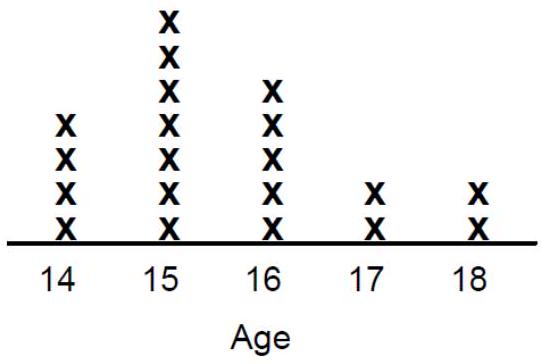
\includegraphics[width=0.40\linewidth]{math-6th/images/f4536730-c0c6-4b8e-8a47-92299a61e85f-1_364_543_2115_1178.jpg}
\end{center}
Find the mean, median, and mode of the data.
\labeledfillin{Mean}{$\approx 15.55$}
\labeledfillin{Median}{$15$}
\labeledfillin{Mode}{$15$}
\begin{solution}
  Mean $\approx 15.55$, median $=15$, mode $=15$ (read counts from the plot to verify).
\end{solution}


\newpage


\question[10]
The ages of a group of friends are listed:
\[
  48,\ 32,\ 29,\ 33,\ 52,\ 48,\ 45,\ 33\text{.}
\]
Find the mean, median, and mode.
\labeledfillin{Mean}{$40$}
\labeledfillin{Median}{$39$}
\labeledfillin{Mode}{$33$ and $48$}
\begin{solution}
  Mean $=40$, median $=39$, modes $=33$ and $48$.
\end{solution}

\question[5]
Marty sent $4$ packages. Their masses were $3\ \mathrm{kg}$, $500\ \mathrm{g}$, $660\ \mathrm{g}$, and $5\ \mathrm{kg}$. What was the approximate average mass of the packages?
\begin{choices}
  \CorrectChoice $2300\ \mathrm{g}$
  \choice $5\ \mathrm{kg}$
  \choice $6500\ \mathrm{g}$
  \choice $3\ \mathrm{kg}$
\end{choices}
\begin{solution}
  Total $\approx 9160\ \mathrm{g}$, mean $\approx 2290\ \mathrm{g}\approx 2300\ \mathrm{g}$.
\end{solution}

\question[10]
This frequency table shows data from accident reports at a traffic police station.
\begin{center}
  \small
  \begin{tabular}{|l|c|}
    \hline
    Length of skid mark (m) & Number of skids \\
    \hline
    $20$ & $13$ \\
    \hline
    $25$ & $22$ \\
    \hline
    $30$ & $24$ \\
    \hline
    $35$ & $44$ \\
    \hline
    $40$ & $43$ \\
    \hline
    $45$ & $54$ \\
    \hline
  \end{tabular}
\end{center}
Find the median of the skid mark lengths. Use that value for $d$ in the formula $s=\sqrt{15d}$ to find the corresponding car speed in meters per second, to the nearest whole number.
\labeledfillin{Median skid length ($d$, in m)}{$35$}
\labeledfillin{Speed $s$ (m/s, nearest whole number)}{$23$}
\begin{solution}
  With $200$ measurements, the median falls in the $35\ \mathrm{m}$ class, so $d=35$. Then $s=\sqrt{15\cdot 35}=\sqrt{525}\approx 23\ \mathrm{m/s}$.
\end{solution}

\endgradingrange{stats}

% \newpage
% \fullwidth{%
%   \vfill
%   \begin{center}
%     \resizebox{\linewidth}{!}{%
%       \partialcombinedgradetable{stats}[h][questions]%
%     }%
%   \end{center}%
% }
